\section{Applying the Linux kernel}

%\subsection{Reverse mapping}

%$$$$$$$$$$$$$$$$$$$$$$$$$$$$$$$$$$$$$$$$$$$$$$$$$$$$$$$$$$$$$$$$$$$$$$$$$$$$$$$$
%Paragraph 1: Linux의 reverse mapping에 대한 자세한 설명 
%$$$$$$$$$$$$$$$$$$$$$$$$$$$$$$$$$$$$$$$$$$$$$$$$$$$$$$$$$$$$$$$$$$$$$$$$$$$$$$$$

The reverse page mapping(rmap), a kernel memory management mechanism, consists
of anonymous rmap and the file rmap.
These two rmap maintains virtual address (VMAs) in order to translate physical
addresses to virtual address[], and the rmaps are a shared global resource.
These global resource of rmap are managed by using a interval tree that means
any processes can update the one.
To protect the shared resource, the Linux kernel uses a semaphore.
This update operations such as tree's insert and remove operation are invoked by
\code{fork()}, \code{exit()} and \code{mmap()}, so simultaneous creation of many
processes causes bottlenecks because not only the update operations can not run
in parallel but also update's lock brings about the cache invalidation traffic.
On the contrary, the rmap rarely reads the tree when it swaps a physical page
out to disk, migrates other cpu, or truncates a file.
Therefore, the Linux rmaps are a update-heavy data structure. 

This section show how to apply LDU to the Linux rmaps to solve the update
serialization problem;it deals with more practical one.

\subsection{Anonymous mapping}

\begin{figure}[tb]
  \begin{center}
     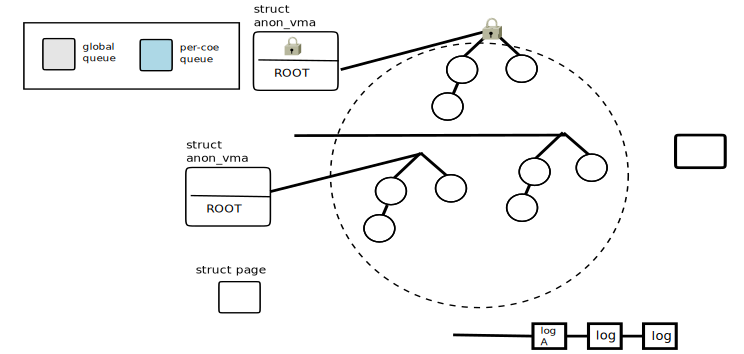
\includegraphics[width=0.5\textwidth,height=0.5\textheight,keepaspectratio]{fig/anon_vma}
  \end{center}
  \caption{An example of applying the \deferu to anonymous reverse mapping. to
  prevent the update operations for the interval tree, the anonymous rmap uses
  the root \code{anon\_vma}'s lock. Therefore, when the child \code{anon\_vma}
  are increased, root lock leads to a scalability bottleneck. LDU global queue
  logs in the position of the root data structure, and the per-core queue also
  logs in the per-core queue with root information.}
  \label{fig:anonvmaramp}
\end{figure}

%$$$$$$$$$$$$$$$$$$$$$$$$$$$$$$$$$$$$$$$$$$$$$$$$$$$$$$$$$$$$$$$$$$$$$$$$$$$$$$$$
%Paragraph 1: linux의 anon vma의 공유된 구조에 대한 설명
%$$$$$$$$$$$$$$$$$$$$$$$$$$$$$$$$$$$$$$$$$$$$$$$$$$$$$$$$$$$$$$$$$$$$$$$$$$$$$$$$
When a process spawns, the parent's \code{anonymous vma chain(AVC)} are copied
to a child, and then the new anonymous vma, indicating the child's AVCs, is
created.
Due to the fact that the continuous process spawns, it becomes more the complex
anonymous rmap data structure;the anonymous ramp is one of the complex data
structure in the Linux kernel[].
Figure \ref{fig:anonvmaramp} shows this complex anonymous rmap data
structure.
To prevent the update operations for the interval tree, the anonymous rmap
uses the root \code{anon\_vma}'s lock. 
Therefore, when the child \code{anon\_vma} are increased, root lock makes lock
contention problem[].

%$$$$$$$$$$$$$$$$$$$$$$$$$$$$$$$$$$$$$$$$$$$$$$$$$$$$$$$$$$$$$$$$$$$$$$$$$$$$$$$$
%Paragraph 2: anon vma에 ldu 적용한 방법에 대한 설명 
%$$$$$$$$$$$$$$$$$$$$$$$$$$$$$$$$$$$$$$$$$$$$$$$$$$$$$$$$$$$$$$$$$$$$$$$$$$$$$$$$
In anonymous ramp, in order to eliminate the problem of lock contention, LDU
adds insert and remove mark field in the \code{AVC} object for concurrent
update, and then it performs the update-side removing logs scheme.
Understanding the log's position of queue header in anonymous rmap is important.
As noted earlier, since the anonymous rmap uses the root lock, LDU global
queue logs in the position of the root data structure, and the per-core queue
also logs in the per-core queue with root information.
LDU does not largely modify the original data structure which show why LDU is a
lightweight method.

\subsection{File mapping}

%$$$$$$$$$$$$$$$$$$$$$$$$$$$$$$$$$$$$$$$$$$$$$$$$$$$$$$$$$$$$$$$$$$$$$$$$$$$$$$$$
%Paragraph 1: linux의 file mapped page reverse mapping의 구조에 대한 설명
%$$$$$$$$$$$$$$$$$$$$$$$$$$$$$$$$$$$$$$$$$$$$$$$$$$$$$$$$$$$$$$$$$$$$$$$$$$$$$$$$
Figure \ref{fig:fileramp} shows the rmap for file.
To translate physical addresses to virtual address, the \code{struct page} for
file rmap indicates the \code{struct address\_space} managed by inode, and
the \code{struct address\_space} manages the VMAs by using the interval tree.
This interval tree is a shared resource between processes, so the Linux uses the
reader-writer semaphore to protect the tree.
The system calls such as \code{fork()}, \code{exit()} and \code{mmap()} entail
a updating VMA associated with file into the interval tree.
When the processes simultaneously invoke \code{fork()}, \code{exit()} and
\code{mmap()} system call, the file rmap also can pose the update serialization
problem.

%$$$$$$$$$$$$$$$$$$$$$$$$$$$$$$$$$$$$$$$$$$$$$$$$$$$$$$$$$$$$$$$$$$$$$$$$$$$$$$$$
%Paragraph 2: file mapping에 ldu 적용한 방법에 대한 설명 
%$$$$$$$$$$$$$$$$$$$$$$$$$$$$$$$$$$$$$$$$$$$$$$$$$$$$$$$$$$$$$$$$$$$$$$$$$$$$$$$$
The LDU can easily be applied to file ramp for eliminating the update
serialization problem.
To use the LDU, the mark fields are added to the \code{struct
vma\_area\_struct}, and the log's queue is added to \code{struct address\_space} or per-core
memory.
For instance, if it uses global queue, the queue header is located in the
\code{struct address\_space}. If not, the queue header is located in the
per-core memory.

In addition, this figure clearly shows why the LDU additionally supports the
global queue because it is a simpler and easier scheme.
For example, consider the global queue, a developer just adds queue header in
the header of original data structure(struct address\_space), and then add mark
field in individual object(struct vma\_area\_struct).
Finally, the developer creates synchronize function and call before the
read.
On the other hand, the per-core queue may need an additional per-core
queue management scheme because the data structure separates between interval
tree head pointer and log's head pointer.

\begin{figure}[tb]
  \begin{center}
     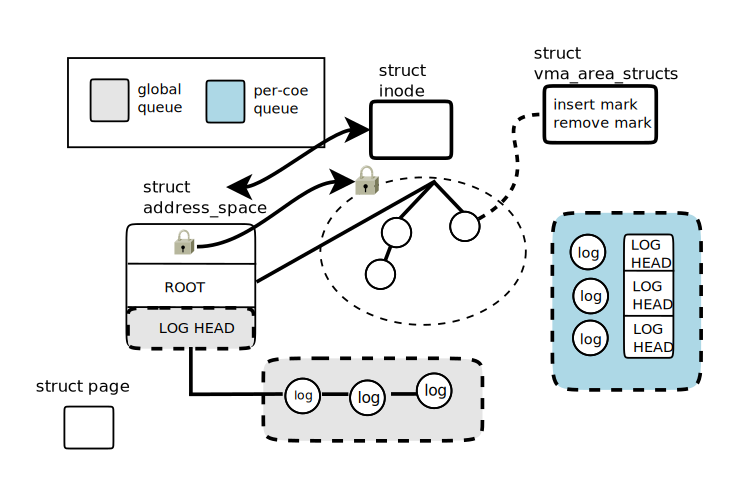
\includegraphics[width=0.5\textwidth,height=0.5\textheight,keepaspectratio]{fig/file_rmap}
  \end{center}
  \caption{An example of applying the \deferu to file reverse mapping. This
   interval tree is a shared resource between processes, so the Linux uses the 
   reader-writer semaphore to protect the tree, so it also becomes a bottleneck.
   to use the LDU, the mark fields are added to the \code{struct
   vma\_area\_struct}, and the log's queue is added to \code{struct
   address\_space} or per-core memory.
}
  \label{fig:fileramp}
\end{figure}

\subsection{Detail Implementation}\label{sec:implementation}

%$$$$$$$$$$$$$$$$$$$$$$$$$$$$$$$$$$$$$$$$$$$$$$$$$$$$$$$$$$$$$$$$$$$$$$$$$$$$$$$$
%Paragraph 1: 커널 버전 및 코드 분량, 테스트에 대한 설명
%$$$$$$$$$$$$$$$$$$$$$$$$$$$$$$$$$$$$$$$$$$$$$$$$$$$$$$$$$$$$$$$$$$$$$$$$$$$$$$$$
We have implemented the new deferred update algorithm in Linux 4.5.rc6 kernel,
and our modified Linux is available as open source. 
%The version of global queue modified code is xx that less complex, but per-core
%queue the modified code is xx-xx.
The implementation is stable enough and has passed virtual memory, scheduler,
and file related testing in the Linux Test Project[1].

%$$$$$$$$$$$$$$$$$$$$$$$$$$$$$$$$$$$$$$$$$$$$$$$$$$$$$$$$$$$$$$$$$$$$$$$$$$$$$$$$
%Paragraph 2: per-core queue 구현에 대한 설명 
%$$$$$$$$$$$$$$$$$$$$$$$$$$$$$$$$$$$$$$$$$$$$$$$$$$$$$$$$$$$$$$$$$$$$$$$$$$$$$$$$
The implementation of per-core queue in the LDU uses per-core hash table that 
can easily distinguish each object.
The LDU per-core hash table implemented as a direct-mapped cache, which one
bucket only has an object because recently used objects will be in the hash
table[Oplog].
When this hash table is met a hash conflict, the LDU evicts the object in the
hash slot located in the per-core memory.
This method is useful when the number of the root objects is small like the file
rmap(\code{struct address\_space}).
Moreover, this method reduce additional tasks of programmers because it can
minimize code modifications and does not need additional locks.
The per-core hash table, however, incurs a hash conflict overhead.
Since the anonymous rmap creates many of child root object(anon\_vma), so it
incurs a hash conflict overhead.
In the case of the anonymous ramp, we do not distinguish object headers to
avoid the hash conflict overhead, but it needs additional tasks with global
lock.
